\section{Strategy to early predict potential failing students}

\label{sec:strategy}

Predicting the potential failing students early is very important in the sense that professors still have enough time to act and avoid students to fail the course. Notice that in case professors act based on the results of our strategy, we can indirectly help on reducing the high rate of failing students. However, in this article, we focus exclusively on identifying these students. This way, evaluating and reporting the rate after applying our strategy is outside the scope of this article.

Our strategy is automatic and objective, consisting of three simple steps: the use of a online judge system, metrics collection, and execution of a well-known clustering algorithm~\cite{hartigan-clustering-algorithms-1975}. Because the strategy is automatic, professors can replicate in their courses, reducing their effort.

Next, we detail the three steps of our strategy to predict the failing students.

\subsection{Online judge system}
% This section should answer: Why is this kind of system important to identify potential falling students?
% Answer: We need metrics. In order to discover how students are performing, it is necessary a close monitoring of students behaviour
% Talk about Huxley, only enough to explain the metrics: submissions and submission_status (Correct ...)

To assess the students performance during a course, it is important to closely monitor them. In this context, metrics represent an alternative to measure their performance. However, retrieving metrics regarding each student is a difficult and time-consuming task. To minimize this problem, one might rely on online learning tools, since these systems are not only a source for these metrics, but allow their automatic retrieval. 

A popular category of this kind of system is the online judges~\cite{uva, sphere}. These systems provide a set of programming problems so that students can submit their solutions. After submitting, the online judge executes the solution against a set of predefined test cases. In case the solution passes over all the tests, the system evaluates the solution as correct. Otherwise, the system evaluates the solution according to the error type (e.g., wrong answer, compilation error, time limit exceeded, runtime error, etc) and even might give important tips so that students can successfully solve the problem afterwards.

Since students only learn how to program by programming~\cite{jenkins-ltsn02}, the online judges consists of an important environment in the sense students can practice and improve their learning process. Also, as the tool is available online, students can find their own rhythms. In addition, online judges play an important role regarding rapid feedback, once professors are often overwhelmed with their daily activities and sometimes are not able to help each student separately.

Given all these advantages, the use of an online judge system is the first step of our strategy. We then can monitor students to automatically identify the candidates to fail the course.

%There always be great students and bad students. The great ones should be presented to challenges that make them even greater and the bad ones should be presented to a different set of problems that allow them to become better. Each programming problem of the Huxley is classified according to this level of difficulty and the programming topics it covers. This allows each student to choose the next problem in accordance with this level of expertise.

% Why the Huxley and not others?
% answer: Metrics and performance improvement (not in scope)

%Sometimes a student misses a basic concept and then cannot follow the next lecture. She believes that there is no going back; the course is behaving at a speed that she thinks she will be not able to follow. Such a student will quickly come to the view that ``they just cannot do programming'', and will attribute this to the perceived difficulty of the subject. In other words, students learn at different speeds. As the tool is available online on the Internet, each student can find its own rhythm.

%In our strategy, we choose to use an online judge named \emph{The Huxley} \cite{paes2013ferramenta} to collect metrics from our students. In this system, the judge provides one of the following outputs for a submission: correct, wrong answer, time limit exceeded, compilation error, runtime error, presentation error and empty answer. We will use these outputs as the main source of metrics. This particular online judge system was chosen because it has some features that we believe will be useful to improve the overall performance of students as a future direction of this research. More specifically, the tool will support us to deal with the following problems:
%\begin{itemize}
%  \item Students only learn how to program by programming~\cite{jenkins-ltsn02}. The Huxley provides a database composed of more than 300 problems. It allows students to submit their solutions to any of these problems and they are encouraged to try once mistakes are not penalized.
%  \item Sometimes a student misses a basic concept and then cannot follow the next lecture. She believes that there is no going back; the course is behaving at a speed that she thinks she will be not able to follow. Such a student will quickly come to the view that ``they just cannot do programming'', and will attribute this to the perceived difficulty of the subject. In other words, students learn at different speeds. As the tool is available online on the Internet, each student can find its own rhythm.

%Acho que esse item nao se encaixa nesse paper.
%  \item Students need rapid feedback. Many professors are overwhelmed with their daily activities. Then they have no time to give feedback on every student code. On the other side, students need this feedback to continue their learning process in the right path. The Huxley provides a feedback right after a student submits her code. The feedback indicates whether the student's code produces the right answer and gives tips otherwise.

%  \item There always be great students and bad students. The great ones should be presented to challenges that make them even greater and the bad ones should be presented to a different set of problems that allow them to become better. Each programming problem of the Huxley is classified according to this level of difficulty and the programming topics it covers. This allows each student to choose the next problem in accordance with this level of expertise.
%\end{itemize}

\subsection{Metrics}

\label{sec:metrics}

The second step of our strategy consists of metrics retrieval. In particular, we retrieve two metrics by using the online judge system. We explain them in what follows:

\begin{itemize}

	\item \textbf{Number of submissions:} this metric represents the number of submissions a student do during the course. Online judge systems commonly provide many problems. To solve a particular one, a student needs to submit at least one correct solution.

	\item \textbf{Number of correct submissions:} if a student solves one problem, we increase this metric by one.

\end{itemize}

Depending on the level of difficulty of a problem, students may submit several times to solve it. However, notice that this is not necessarily a bad thing regarding the learning process. For example, submitting many times means that students are somehow practicing and studying continuously. Thus, although she is not hitting a right solution, she is trying hard and will eventually hit one. Thus, the number of submissions metric is a good indicator of the amount of practice, which is frequently associated with the level of engaging and learning. However, when considered isolated, a high number of submissions may also mean that the student is getting frustrated due to so many wrong answers she receives. This way, we also consider the number of correct submissions to compensate and help us on studying such cases as well.

\todo{Referencia do porque as metricas sao boas: quanto menos exercicio, maior a probabilidade de levar pau.}

\subsection{Clustering algorithm}

To identify potential failing students, we use an existing clustering algorithm~\cite{hartigan-clustering-algorithms-1975} to define groups of students. Our idea consists of identifying different groups of students so we can clearly separate students susceptible to fail from the other ones. To compute the groups, the algorithm takes into account the metrics we present in Section~\ref{sec:metrics}. To make the strategy parameterizable in terms of number of groups, we use the well-known clustering algorithm k-means~\cite{k-means-1979}, which takes such a number as input.

Notice that the number of groups plays an important role on identifying potential failing students. In this article, we set the algorithm to compute two and three groups and evaluate both cases. For two groups, we have students who will either fail or pass. For three groups, we have fail, pass, and students in which the strategy will not conclude anything about them, which we name ``inconclusive.'' This is reasonable since our study focuses on the very first 30 days, which means our drawings regarding the inconclusive group might be completely wrong: these students can either improve themselves and pass the course or fail due to several reasons.

We focus on two and three groups basically for two reasons: (i) using one group is useless; and (ii) more than three only brings more inconclusive groups to the table which, given our context, is pretty much the same of having only one inconclusive group.

\subsection{Summary}

Figure~\ref{fig:strategy} combines all steps of our strategy. Notice that our strategy is general in the sense we can use any online judge system, as long as we can collect the metrics we use from the system.

%, as long as we can collect the metrics we consider, we can use any online judge system.

To instantiate our strategy, we use the online judge system named \textit{Huxley}~\cite{paes2013ferramenta}. The system is available online only in portuguese at \url{http://www.thehuxley.com/}. It provides a database composed by more than 300 problems classified according to level of difficulty and programming topics. This allows the students to choose the next problem in accordance to their corresponding levels. Notice that this helps on avoiding misleading in our metrics, e.g., many incorrect submissions to a problem that the student is not able to solve yet.

%and students are encouraged to use the system, once there is absolutely no penalty in case of wrong solutions.

%Huxley also classifies the problems according to level of difficulty and programming topics. This allows the students to choose the next problem in accordance to their corresponding levels.

%As the classes are happening, we encourage students to solve the problems available at Huxley. Although solving exercises is not mandatory, there are some particular activities where the professor forces students to use Huxley, such as formal exams.

Next, we collect the metrics we detail in Section~\ref{sec:metrics}. To identify potential failing students \textit{early}, we collect the metrics for the first 30 days (representing 25\% of the semester) of the introductory programming courses. Then, we execute the k-means clustering algorithm.

\begin{figure}[htb]
\centering
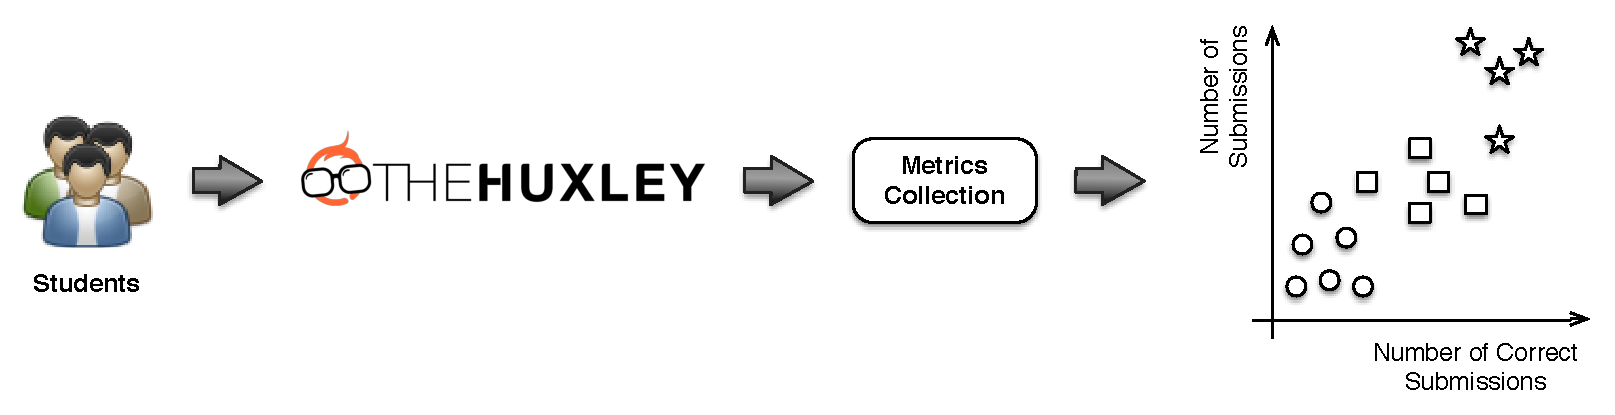
\includegraphics[width=1.0\textwidth,natwidth=610,natheight=642]{images/Strategy.pdf}
\caption{Summary of our strategy to identify potential failing students.}
\label{fig:strategy}
\end{figure}

We illustrate the groups using shapes in Figure~\ref{fig:strategy}. In this particular case, we set k-means to compute three different groups. The circles represent the students candidates to fail the course. Notice that they submitted few solutions and few of them are correct.

%\todo{Como deixar a estrategia mais geral? Dizer que pode ser qualquer online judge desde que tenha as metricas? Dizer que e mais geral e que instanciamos a estrategia com o huxley.}